Auf Grundlage der zuvor genannten Messvoraussetzungen konnte die Roboter-Gesten-Anwen-\\dung verschiedenen Tests unterzogen und deren Ergebnisse ausgewertet werden. Zur Durchführung der Tests wurde die Roboter-Gesten-Anwendung mit zusätzlichen \quoteMark{*\_MEASUREMENT}-Flags, zu denen die Flags \quoteMark{GESTURE\_MEASUREMENT}, \quoteMark{COMMUNICATION\_MEASU-\\REMENT} und \quoteMark{POSITION\_MEASUREMENT} zählen, kompiliert um ausführliche Statistikdaten für den jeweils durchgeführten Testfall zu erhalten. Die durchgeführten Tests reichen hierbei von Latenztests der Gestenerkennung mittels der Azure Kinect über Latenztests der Kommunikation mittels ROS und der direkten Kommunikation mit dem \quoteMark{WidowX 200}-Lernroboter bis hin zu der Genauigkeit der anzufahrenden Zielpositionen. Die erhobenen statistischen Daten wurden analysiert und werden nachfolgend mittels Diagrammen veranschaulicht und kritisch hinterfragt.

% Implementierung: Roboter wählt seine eigene Bahn
% Bewegen durch Gesten in beliebigen Koordinatensystemen mit unterschiedlichen Orientierungen

% Wie lange benötige ich für das Teachen mittels Gesten? Ist es ein vertretbarer Aufwand? Was ist ein vertretbarer Aufwand?

% Hierfür wurde darauf geeinigt, dass die Bewegungsabläufe des Roboters auch nachträglich nachbearbeitet werden können.

% Wünschenswert, die Bewegungen können jedoch aber im nachhinein auch nachträglich nachbearbeitet werden. Wenige mm wären ideal, aber wenige cm würden auch genügen.

% ------------

% Azure Kinect: Belichtungszeit: 1,6 ms bis zu 20,3 ms (https://docs.microsoft.com/en-us/azure/kinect-dk/hardware-specification) -> TODO: Passive IR einschalten?
% Realsens: Belichtungszeit: 900 ns (https://www.imveurope.com/press-releases/intel-realsense-lidar-depth-camera-l515) (https://softei.com/framos-claims-hi-res-intel-realsense-lidar-depth-camera-is-worlds-smallest/) (https://venturebeat.com/2019/12/11/intels-new-realsense-camera-packs-a-lidar-sensor-for-enhanced-depth-perception/) -> Distanz?
% https://www.intelrealsense.com/compare-depth-cameras/
% https://www.intelrealsense.com/depth-camera-d435/

% https://docs.microsoft.com/en-us/windows/mixed-reality/ISSCC-2018



%----------------

% https://feedback.azure.com/forums/920053-azure-kinect-dk/suggestions/38129473-body-tracking-without-cudnn
% https://feedback.azure.com/forums/920053-azure-kinect-dk/suggestions/39945454-legacy-body-tracking-like-kinect-v2
% https://github.com/microsoft/Azure-Kinect-Sensor-SDK/issues/1080



%-----------
% konkrete Aussage zur Performanz, Stabilität, Modularität, Hohe Skalierbarkeit,
% Erweiterbarkeit

% Erfahrungen

% Mögliche Prognosen

% Limitierungen

% Entwicklungswerkzeuge


% --------------

% weiche Echtzeitfähigkeit
% Durchsatz, Latenzen, ...

% Die Gestensteuerung des WidowX 200, welches auf dem für diese Arbeit erstellten Roboter-Gesten-Framework basiert und als Basis für andere gestengesteuerte Roboter dienen kann, wird auf die Ergonomie, Echtzeitfähigkeit, Genauigkeit der Gestenerkennung und Genauigkeit der Zielpositionen hin überprüft. Zudem wird ROS 1 auf die Netzwerklatenz hin überprüft um darauf basierend eine Einschätzung zu gegeben ob sich ROS 1 für echtzeitfähige Systeme eignet.

\section{Latenz der Gestenerkennung}
Zum Testen der Latenz der Gestenerkennung wurde das Azure Kinect Body Tracking SDK im CPU-Modus anstatt mit der Grafikkartenbeschleunigung gestartet. Dies war notwendig, da eine Grafikkarte von AMD statt einer Nvidia Grafikkarte im Testsystem eingesetzt wird. Zudem kann hiermit der kleinste gemeinsame Nenner der im Umlauf befindlicher Systeme widergespiegelt werden, welche keine propritären Features, wie z.B. CUDA, von Nvidia Grafikkarten verwenden. Als alternative und platformunabhängige Programmierschnittstelle zu CUDA wäre hier z.B. OpenCL oder Vulkan anzumerken \cite{vulkan_api_2020}. Die Latenz der Gestenerkennung beinhaltet die Zeit vom Aussenden des Infrarot-Lichtimpuls bis zum Empfang und Absorption des Lichtimpuls bis hin zur Latenz über das \quoteMark{USB 3.0}-Kabel und der Verarbietung der Daten durch das Azure Kinect Body Tracking SDK. Zum Testen der Latenz der Gestenerkennung wurde die Roboter-Gesten-Anwendung und deren Abhängigkeiten mittels der Flags \quoteMark{MEASUREMENT} und \quoteMark{GESTURE\_MEASUREMENT}, welche im Anhang \ref{appendix1.2:Installation_und_Konfiguration_der_Pakete} aufgezeigt werden, kompiliert. Bei der Durchführung des Tests wurden von dem Proband die in dieser Arbeit entwickelten Gesten abwechselnd in zufälliger Reihenfolge vor der Azure Kinect ausgeführt. Die Datei \quoteMark{Messung der Gestenerkennung.csv}, welche bei der Durchführung des Tests von der Roboter-Gesten-Anwendung erstellt wurde, ist auf der CD/ISO im Verzeichnis \quoteMark{Testdaten/} zu finden.

\begin{figure}[htb]
	\centering
	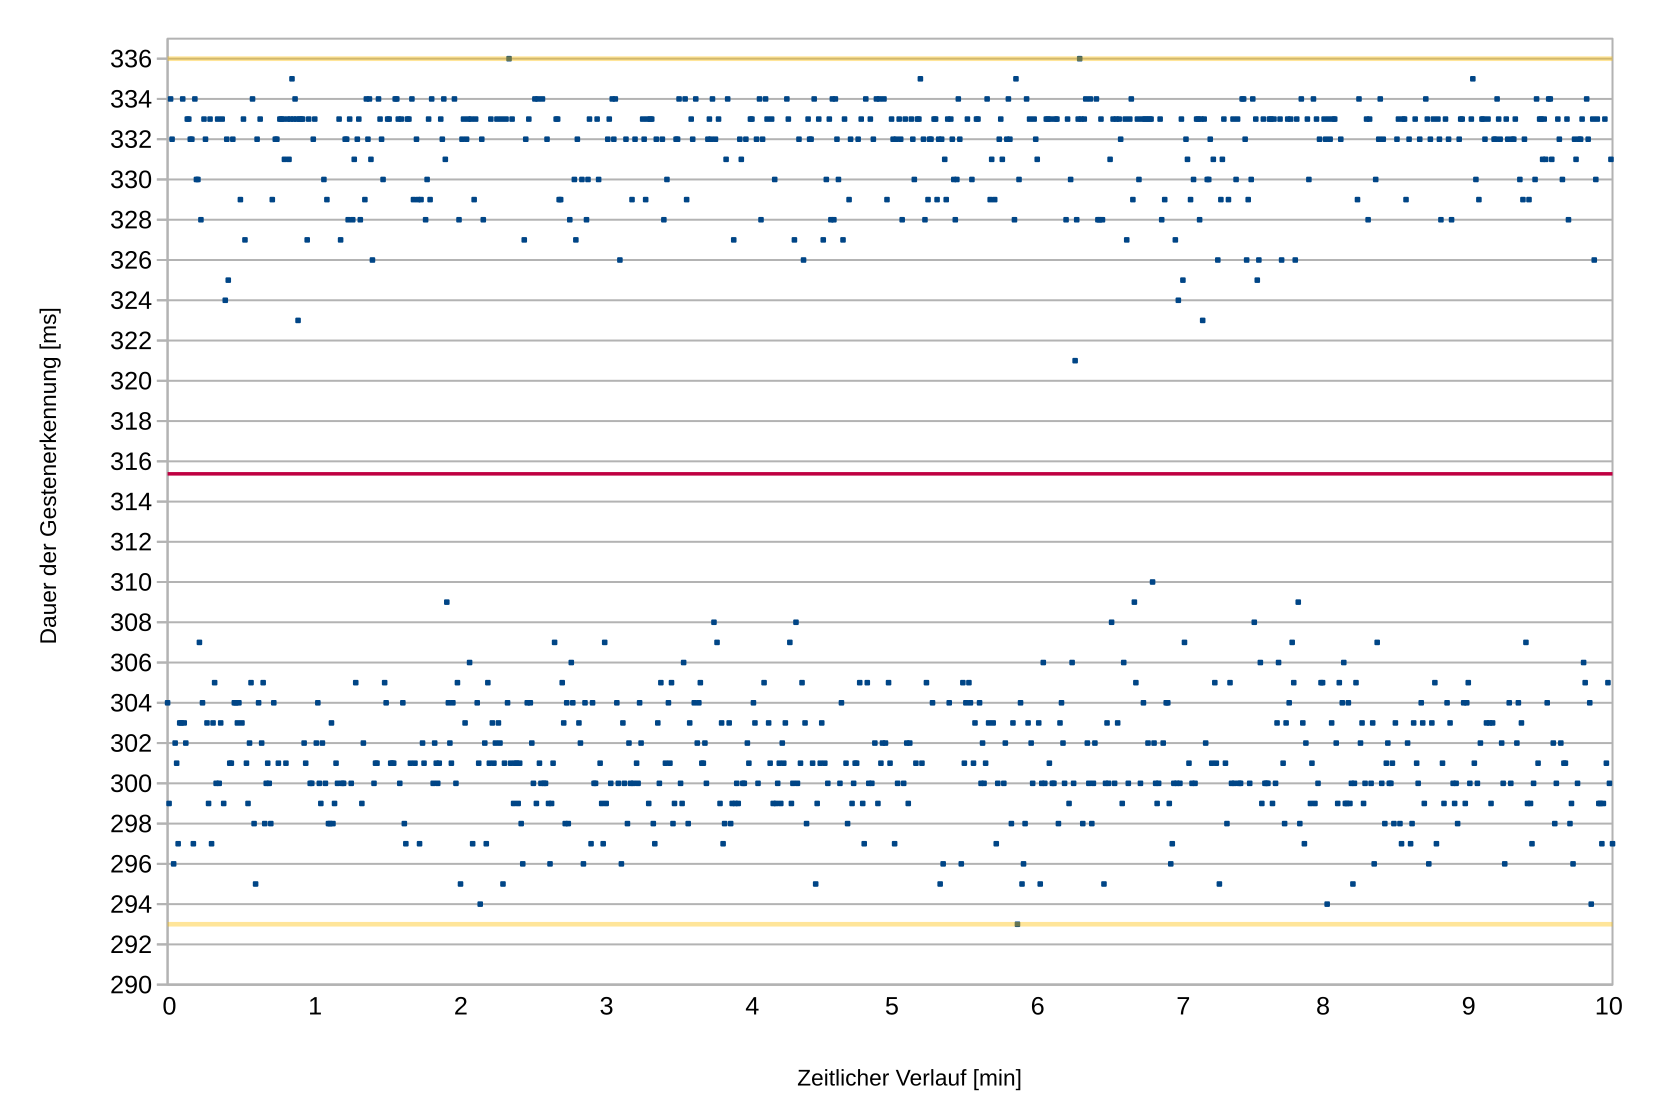
\includegraphics[width=1.04\textwidth]{images/ergebnisse/dauer_der_gestenerkennung_verlauf}
	\caption[Zeitlicher Latenzverlauf der Gestenerkennung der Azure Kinect]{Zeitlicher Latenzverlauf der Gestenerkennung der Azure Kinect\\Quelle: Eigene Ausarbeitung}
	\label{fig:measurement_gesture_recognition_azure_kinect}
\end{figure}
\FloatBarrier

In Abbildung \ref{fig:measurement_gesture_recognition_azure_kinect} ist zu sehen, dass der Mittelwert der Gestenerkennungsdauer, welcher durch die hellrote Linie visualisiert wird, in Richtung \num{326,29} ms tendiert. Die minimale Dauer der Gestenerkennung, welche durch die untere orange Linie visualisiert wird, beträgt \num{291} ms. Die maximale Dauer der Gestenerkennung, welche durch die obere orange Linie visualisiert wird, beträgt hingegen \num{366} ms. Die violette Linie stellt die Tendenz der Gestenerkennungsdauer dar, welche jedoch gleich zu bleiben scheint. Anzumerken ist, dass die Gestenerkennungsdauer sich im Durchschnitt stabil im Bereich zwischen \num{314,02} ms und \num{338,55} ms bewegt. Die annähernd gleich bleibende Gestenerkennungsdauer kann auf das DNN des Azure Kinect Body Tracking SDKs und den eingesetzten Prozess-Scheduler zurückgeführt werden. Eine nichtdeterministische Berechnung würde hierbei vermehrt Spikes und unvorhersagbarere Änderungen bei der Gestenerkennungsdauer bewirken. Nichtsdestotrotz liegen diese Werte weit über den 50 ms, welches für ein Teach Pendant empfohlen wird \cite[55]{prassler_advances_2004}. Zudem ist eine Verzögerung der Gestenerkennung bei über 100 ms für die bedienende Person bereits deutlich spürbar \cite{miller_response_1968}.

\section{Latenz der Roboter-Kommunikation mit und ohne ROS-Anbindung}
Zum Testen der Latenz der Roboter-Kommunikation mit und ohne ROS-Anbindung wurde bei der direkten Kommunikation zum Roboter die Latenz zwischen der aufrufenden Roboter-Gesten-Anwendung und der InterbotiX-Schnittstelle gemessen. Bei der ROS-Anbindung wird die Latenz der Kommunikation zwischen der Roboter-Gesten-Anwendung über den TCP/IP-Stack und daher über das Netzwerk bis hin zu der InterbotiX-Schnittstelle analysiert und gemessen. Bei der Untersuchung der Netzwerklatenz werden verschiedene praxisnahe Netzwerkkonstellationen simuliert um unvorhergesehene Netzwerklatenzen auffinden und diesen gegebenenfalls entgegenwirken zu können. Die Tests werden in einem Gigabit-Ethernet-Netzwerk durchgeführt, da Gigabit-Ethernet zum Zeitpunkt der Veröffentlichung dieser Arbeit als Standard angesehen wird und bereits weit bei Routern und Clientsystemen verbreitet ist \cite{gigabit_ethernet_2020}.\\

Zur Simulation der Netzwerkumgebungen wird NetEm mit Token Bucket Filter eingesetzt. NetEm stellt ein Netzwerkemulator dar und der Token Bucket Filter kann eine Warteschlange simulieren. Mithilfe von NetEm und Token Bucket Filter können verschiedene Netzwerkschnittstellen emuliert werden. Hierzu werden die im Linux-Kernel vorhandenen Möglichkeiten zur Steuerung des Netzwerkverkehrs eingesetzt. Bei ausgehenden Paketen können so Verzögerungen, Paketverlust, Duplizierung, Datenratenlimits und weitere Merkmale emuliert werden um eine Netzwerkschnittstelle an die Gegebenheiten eines vorhandenen Netzwerks anzupassen und z.B. Tests ohne die reale Netzwerkhardware reproduzierbar zu machen \cite{hemminger_network_nodate}. Ein Gigabit-Ethernet-Netzwerk, welches mit einem Router verbunden ist, kann wie in Listing \ref{lst:network_emulation_with_net_em} simuliert werden.\newline\vspace{-1.0em}

\begin{lstlisting}[style=bash, caption={Gigabit-Ethernet-Netzwerkemulation mit NetEm und Token Bucket Filter}, label={lst:network_emulation_with_net_em}]
sudo tc qdisc add dev lo root handle 1: tbf rate 940Mbit burst 8192 limit 16384
sudo tc qdisc add dev lo parent 1:1 handle 10 netem corrupt 0.5% loss 0.1% delay \
0.2ms 0.05ms distribution normal reorder 3% 50%
\end{lstlisting}\leavevmode\newline\vspace{-1.0em}

In Listing \ref{lst:network_emulation_with_net_em} wird das Kommandozeilenprogramm \quoteMark{tc} verwendet um auf die Funktionalitäten von NetEm und des Token Bucket Filters zugreifen zu können. Zur Verwendung von \quoteMark{tc} werden Administratorrechte benötigt, da mit diesem Tool grundlegende Netzwerkeigenschaften, wie z.B. Datenraten, verändert werden können. \quoteMark{qdisc} ist die Abkürzung für \quoteMark{Queueing Discipline} und stellt den Scheduler dar, welcher die Netzwerkpakete entgegennimmt. Mit \quoteMark{add dev} kann ein Netzwerkinterface hinzugefügt werden. In diesem Fall wird \quoteMark{lo}, welches das Loopback-Interface darstellt und über \quoteMark{localhost} oder \quoteMark{127.0.0.1} angesprochen werden kann, ausgewählt. \quoteMark{root} und \quoteMark{parent} stellen dabei Klassen dar, wobei einer \quoteMark{root}-Klasse eine \quoteMark{parent}-Klasse zugewiesen werden kann. Daher wird in Listing \ref{lst:network_emulation_with_net_em} über \quoteMark{parent 1:1} das erste verfügbare Element des \quoteMark{root}-Elements zugewiesen. Mit der Option \quoteMark{handle} wird ein Bezeichner zugewiesen über den die jeweilige Klasse angesprochen werden kann. Hierbei ist die Option \quoteMark{handle 1:} gleichbedeutend mit der Option \quoteMark{handle 1:0} und daher kann auch über die Option \quoteMark{parent 1:1} auf die \quoteMark{root}-Klasse zugegriffen werden. Die Optionen \quoteMark{tbf} und \quoteMark{netem} spezifizieren den Toket Bucket Filter oder NetEm. Mit \quoteMark{rate} kann die maximale Datenrate des Netzwerkinterface angegeben werden \cite{tc_net_em_nodate}. Bei einem Gigabit-Ethernet-Netzwerk kann hierbei eine Nettorate von 940 Mbit/s erreicht werden \cite{datendurchsatz_2020}. Die Option \quoteMark{burst} gibt an wie viele Bytes an Daten im Schnellzugriffs-Buffer gehalten werden können und die Option \quoteMark{limit} gibt an wie viele Bytes an Daten in der Warteschlange gehalten werden können bis diese gesendet werden können \cite{tc_net_em_nodate}. Bei Gigabit-Ethernet ist ein Burst von 8192 Bytes und ein Limit von 16384 Bytes möglich \cite{dembowski_lokale_2007}. Mit der Option \quoteMark{corrupt} kann die Anzahl fehlerhaften Pakete in Prozent angegeben werden. Die Option \quoteMark{loss} gibt an wie viele Pakete in Prozent über das Netzwerk verloren gehen. Eine Verzögerung kann mit dem ersten Argument und eine Schwankung mit dem zweiten Argument von der Option \quoteMark{delay} spezifiziert werden. Eine Verteilungsfunktion kann dazu genutzt werden um eine der Verteilung ähnelnde Verzögerung zu erreichen. Die Pakete können zudem mit der Option \quoteMark{reorder} neu angeordnet werden um verspätete Netzwerkpakete zu simulieren. Das erste Argument der Option \quoteMark{reorder} gibt die Anzahl der neu anzuordnenden Pakete und das zweite Argument die Korrelation in Prozent an \cite{tbf_token_bucket_filter_nodate}. Bei Gigabit-Ethernet und einem Router dazwischen ist eine Fehlerrate von \num{0,5}\%, eine Verlustrate von \num{0,1}\%, eine Verzögerung von \num{0,2} ms mit einer Schwankung von \num{0,05} ms und einer normalverteilten Verzögerung realitätsnah. Eine Neuanordnung der Netzwerkpakete von 3\% mit einer Korrelation von 50\% stellt eine praxisnahe Annäherung an die Gegebenheiten eines Gigabit-Ethernet-Netzerks mit Routeranbindung dar \cite{admin_understanding_2018}.\\

Bei der Durchführung der Tests wurden von dem Proband die in dieser Arbeit entwickelten Gesten abwechselnd in praxinaher Reihenfolge vor der Azure Kinect ausgeführt um die Latenz der Kommunikation an einem praxisnahen Testbeispiel zu testen. Die Tests wurden zuerst an dem Loopback-Interface ohne den in Listing \ref{lst:network_emulation_with_net_em} angegeben Beschränkungen getestet um eine lokale Interprozesskommunikation mithilfe des TCP/IP-Stacks zu testen. Anschließend wurden die in Listing \ref{lst:network_emulation_with_net_em} angegebenen Beschränkungen an drei verschiedenen Netzwerkkonstellationen angewandt. Die Netzwerkkonstellationen schließt hierbei eine Netzwerksimulation ohne zusätzlichen Netzwerktraffic und eine Netzwerksimulation mit hohem Netzwerktraffic mit ein um die zwei Randfälle testen zu können. Bei der Netzwerksimulation mit hohem Netzwerktraffic werden drei 4K-ROS-Nodes simuliert um das Gigabit-Ethernet-Netzwerk mit einer Datenrate 1176 MB/s an seine maximale Grenze und darüber hinaus zu bringen. Dies stellt sicher, dass das Testnetzwerk voll zu jederzeit voll ausgelastet ist. Zum Testen der Latenz der Roboter-Kommunikation mit und ohne ROS-Anbindung wurde die Roboter-Gesten-Anwendung und deren Abhängigkeiten zudem mittels der Flags \quoteMark{MEASUREMENT} und \quoteMark{COMMUNICATION\_MEASUREMENT}, welche im Anhang \ref{appendix1.2:Installation_und_Konfiguration_der_Pakete} aufgezeigt werden, kompiliert. Die Dateien für diesen Test, welche von der Roboter-Gesten-Anwendung erstellt wurden, sind in den jeweiligen Unterordnern \quoteMark{Messung der direkten Kommunikation}, \quoteMark{ROS (App \& keine Netzwerksimulation)}, \quoteMark{ROS (App \& mit Netzwerksimulation)} und \quoteMark{ROS (App mit Netzwerksimulation \& hohe Auslastung)} auf der CD/ISO im Verzeichnis \quoteMark{Testdaten/Messung der Kommunikation/} zu finden.

\begin{figure}[htb]
	\centering
	\includegraphics[width=1.04\textwidth]{images/ergebnisse/Messung_der_direkten_Kommunikation}
	\caption[Zeitlicher Latenzverlauf der direkten Kommunikation des \quoteMark{WidowX 200}-Lernroboters]{Zeitlicher Latenzverlauf der direkten Kommunikation des \quoteMark{WidowX 200}-Lernroboters\\Quelle: Eigene Ausarbeitung}
	\label{fig:measurement_robot_direct_communication}
\end{figure}
\FloatBarrier

\textcolor{red}{TODO}

\begin{figure}[htb]
	\centering
	\includegraphics[width=1.04\textwidth]{images/ergebnisse/Messung_der_ROS_Kommunikation_App_und_keine_Netzwerksimulation}
	\caption[Zeitlicher Latenzverlauf der ROS-Kommunikation des \quoteMark{WidowX 200}-Lernroboters (ohne Netzwerksimulation)]{Zeitlicher Latenzverlauf der ROS-Kommunikation des \quoteMark{WidowX 200}-Lernroboters (ohne Netzwerksimulation)\\Quelle: Eigene Ausarbeitung}
	\label{fig:measurement_robot_ros_without_network_simulation}
\end{figure}
\FloatBarrier

\textcolor{red}{TODO}

\begin{figure}[htb]
	\centering
	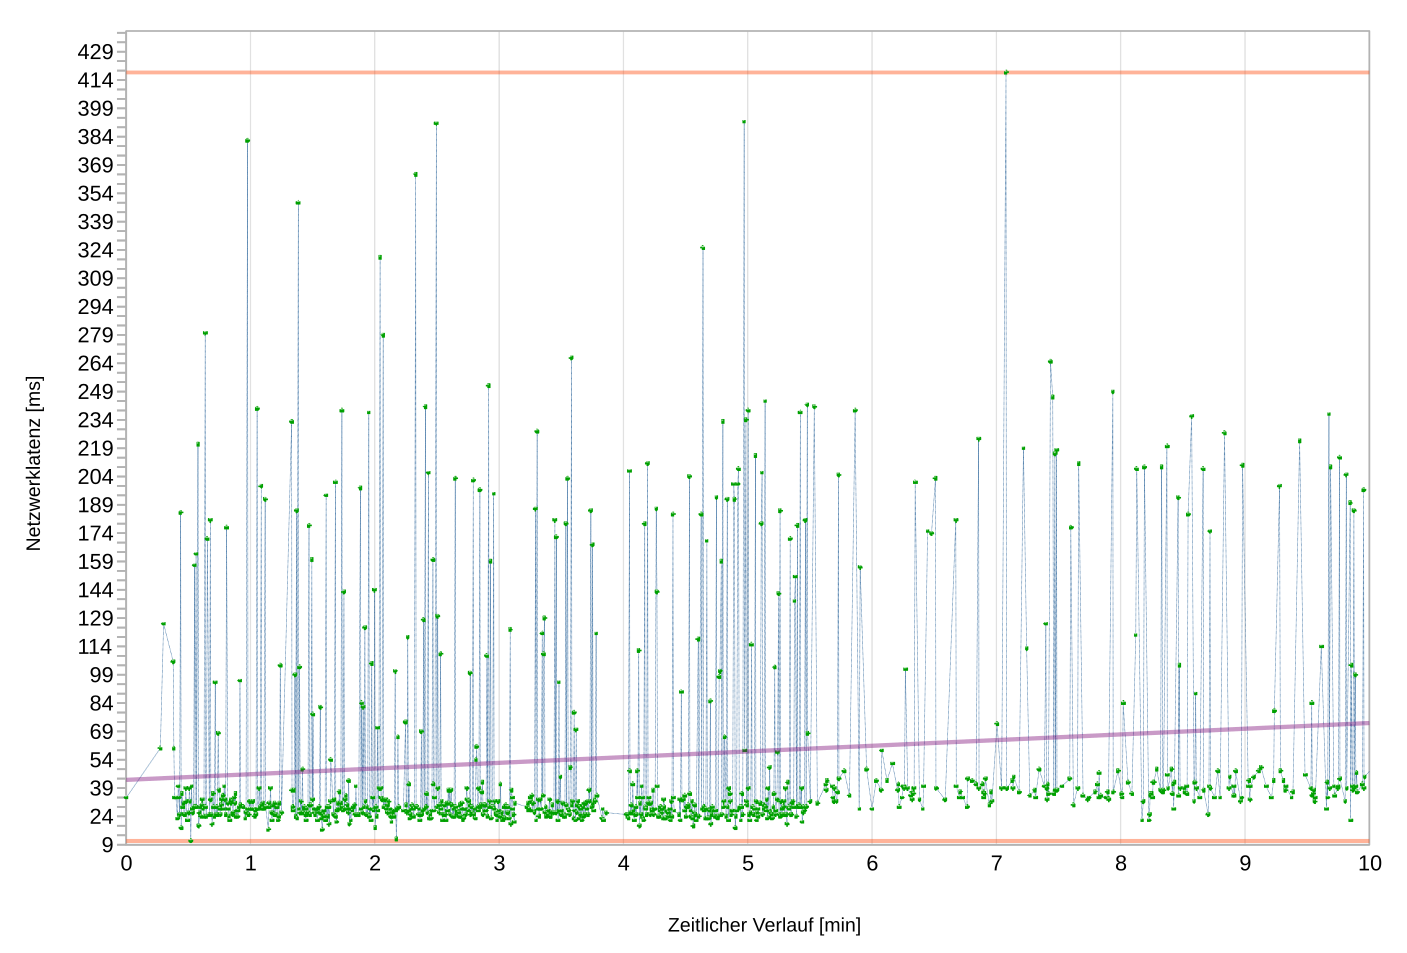
\includegraphics[width=1.04\textwidth]{images/ergebnisse/ROS_App_und_mit_Netzwerksimulation}
	\caption[Zeitlicher Latenzverlauf der ROS-Kommunikation des \quoteMark{WidowX 200}-Lernroboters (mit Netzwerksimulation, geringe Netzwerkauslastung)]{Zeitlicher Latenzverlauf der ROS-Kommunikation des \quoteMark{WidowX 200}-Lernroboters (mit Netzwerksimulation, geringe Netzwerkauslastung)\\Quelle: Eigene Ausarbeitung}
	\label{fig:measurement_robot_ros_with_network_simulation_low_network_traffic}
\end{figure}
\FloatBarrier

\textcolor{red}{TODO}

\begin{figure}[htb]
	\centering
	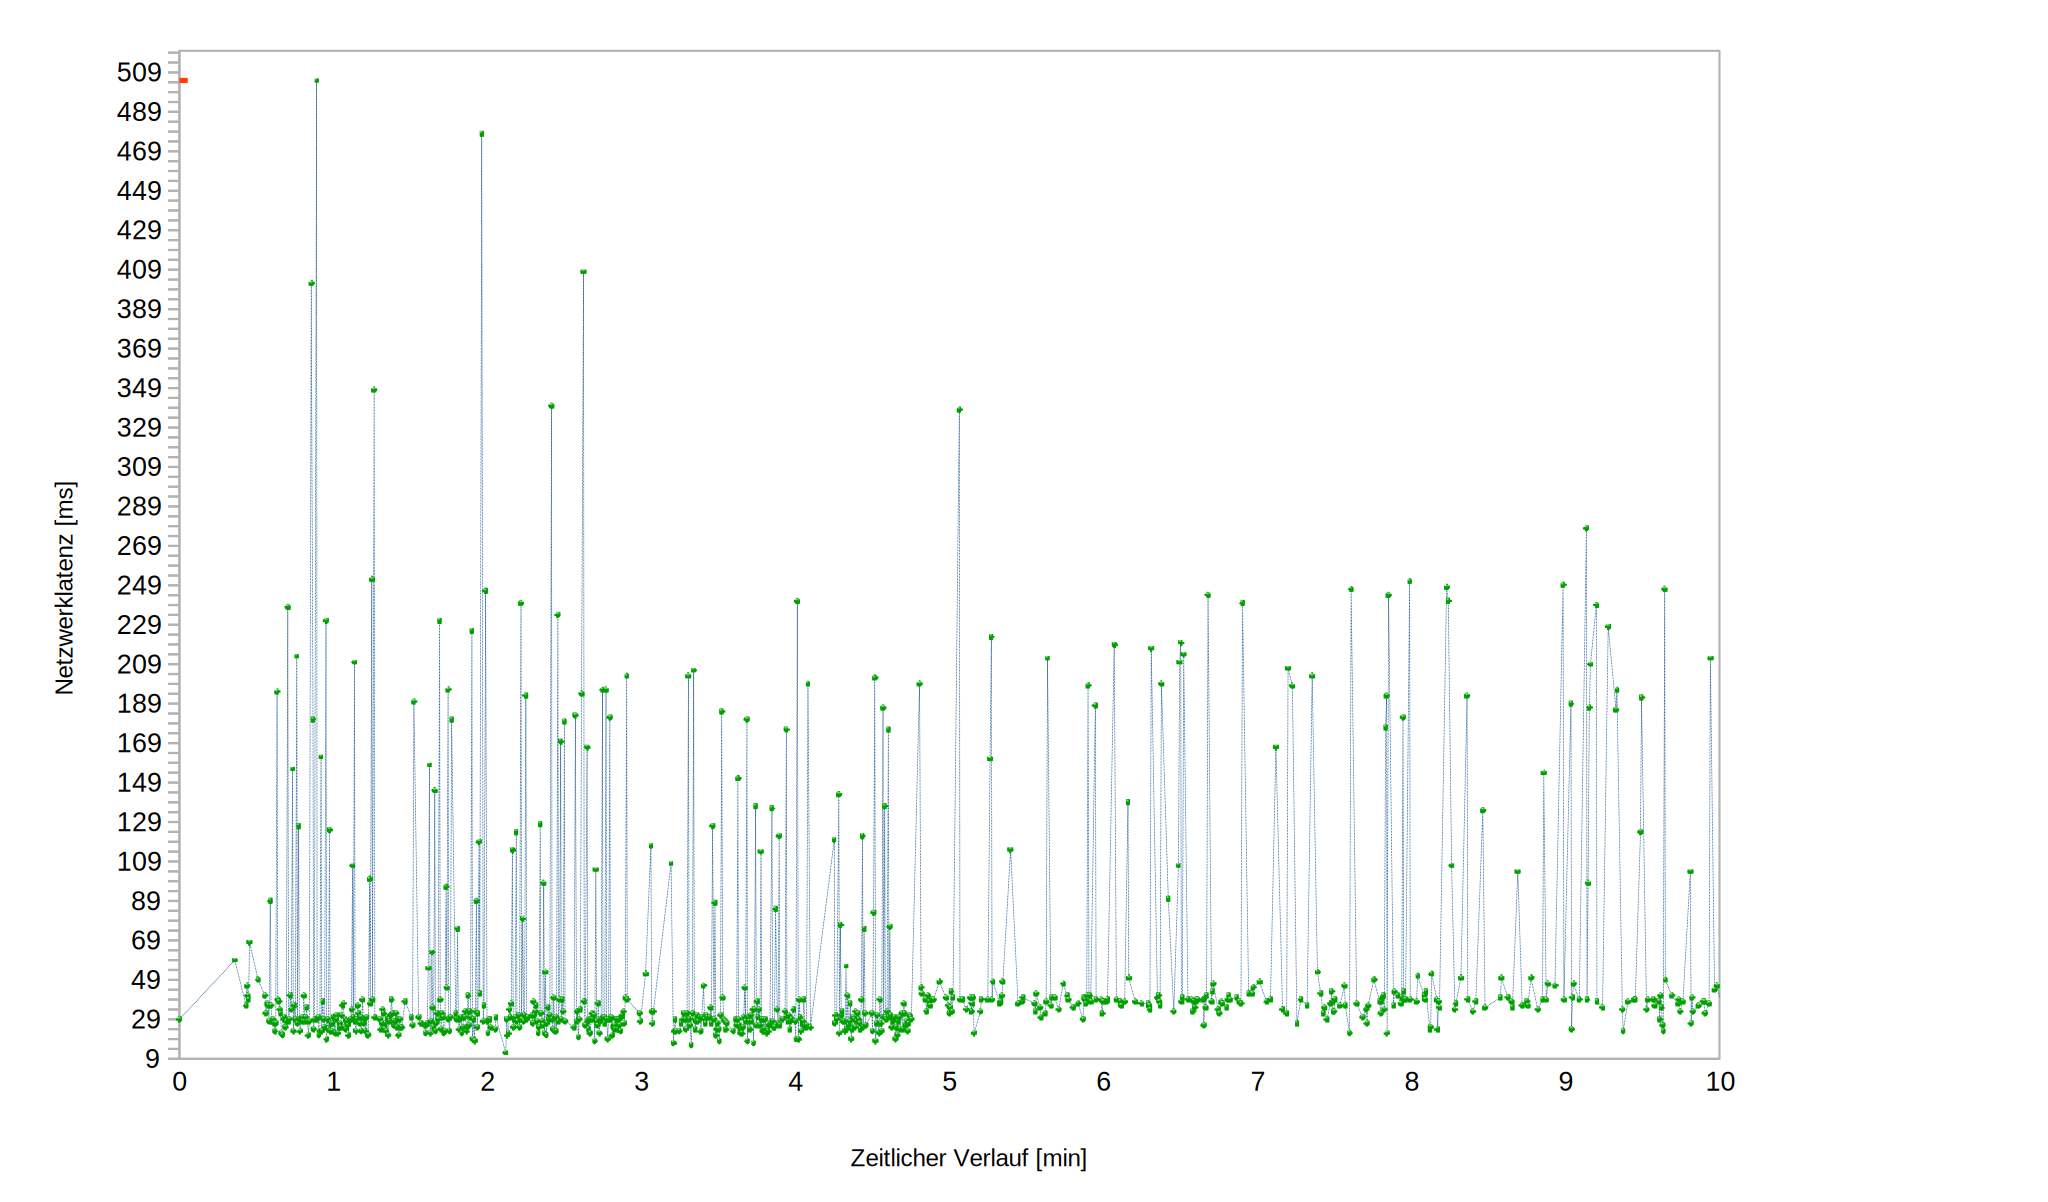
\includegraphics[width=1.04\textwidth]{images/ergebnisse/ROS_App_mit_Netzwerksimulation_und_hohe_Auslastung}
	\caption[Zeitlicher Latenzverlauf der ROS-Kommunikation des \quoteMark{WidowX 200}-Lernroboters (mit Netzwerksimulation, hohe Netzwerkauslastung)]{Zeitlicher Latenzverlauf der ROS-Kommunikation des \quoteMark{WidowX 200}-Lernroboters (mit Netzwerksimulation, hohe Netzwerkauslastung)\\Quelle: Eigene Ausarbeitung}
	\label{fig:measurement_robot_ros_with_network_simulation_high_network_traffic}
\end{figure}
\FloatBarrier

\textcolor{red}{TODO}

\section{Genauigkeit der Zielpositionen}
Zur Genauigkeitsmessung der Zielpositionen werden diese im Simulator Gazebo durchgeführt. In der Simulationsumgebung wurde ein virtueller Raum erschaffen, in welchem die Zielpositionen bereits genau vordefiniert sind. Die ermittelten Positionen können daraufhin mit den exakten Positionen verglichen werden um so genaue Differenzen bestimmen zu können.

Für diesen Testfall wurde die Roboter-Gesten-Anwendung und deren Abhängigkeiten mittels der Flags \quoteMark{MEASUREMENT} und \quoteMark{POSITION\_MEASUREMENT}, welche im Anhang \ref{appendix1.2:Installation_und_Konfiguration_der_Pakete} aufgezeigt werden, kompiliert.

\textcolor{red}{TODO}

% Wie genau kommt man ans gewünschte Ziel? (Einheit: mm)
% Wie viele Korrekturen braucht ein Proband um am nächsten ans gewünschte Ziel zu kommen?

% In einer realen Umgebung nur mit Ungenauigkeiten messbar
%In einer Simulationsumgebung (z.B. Gazebo) kann die Distanz genau und automatisiert gemessen werden
%Visualisierung:
%  *Diagramme
%  *    Mittelwert, die Standardabweichung, Varianz, ...

\begin{figure}[htb]
	\centering
	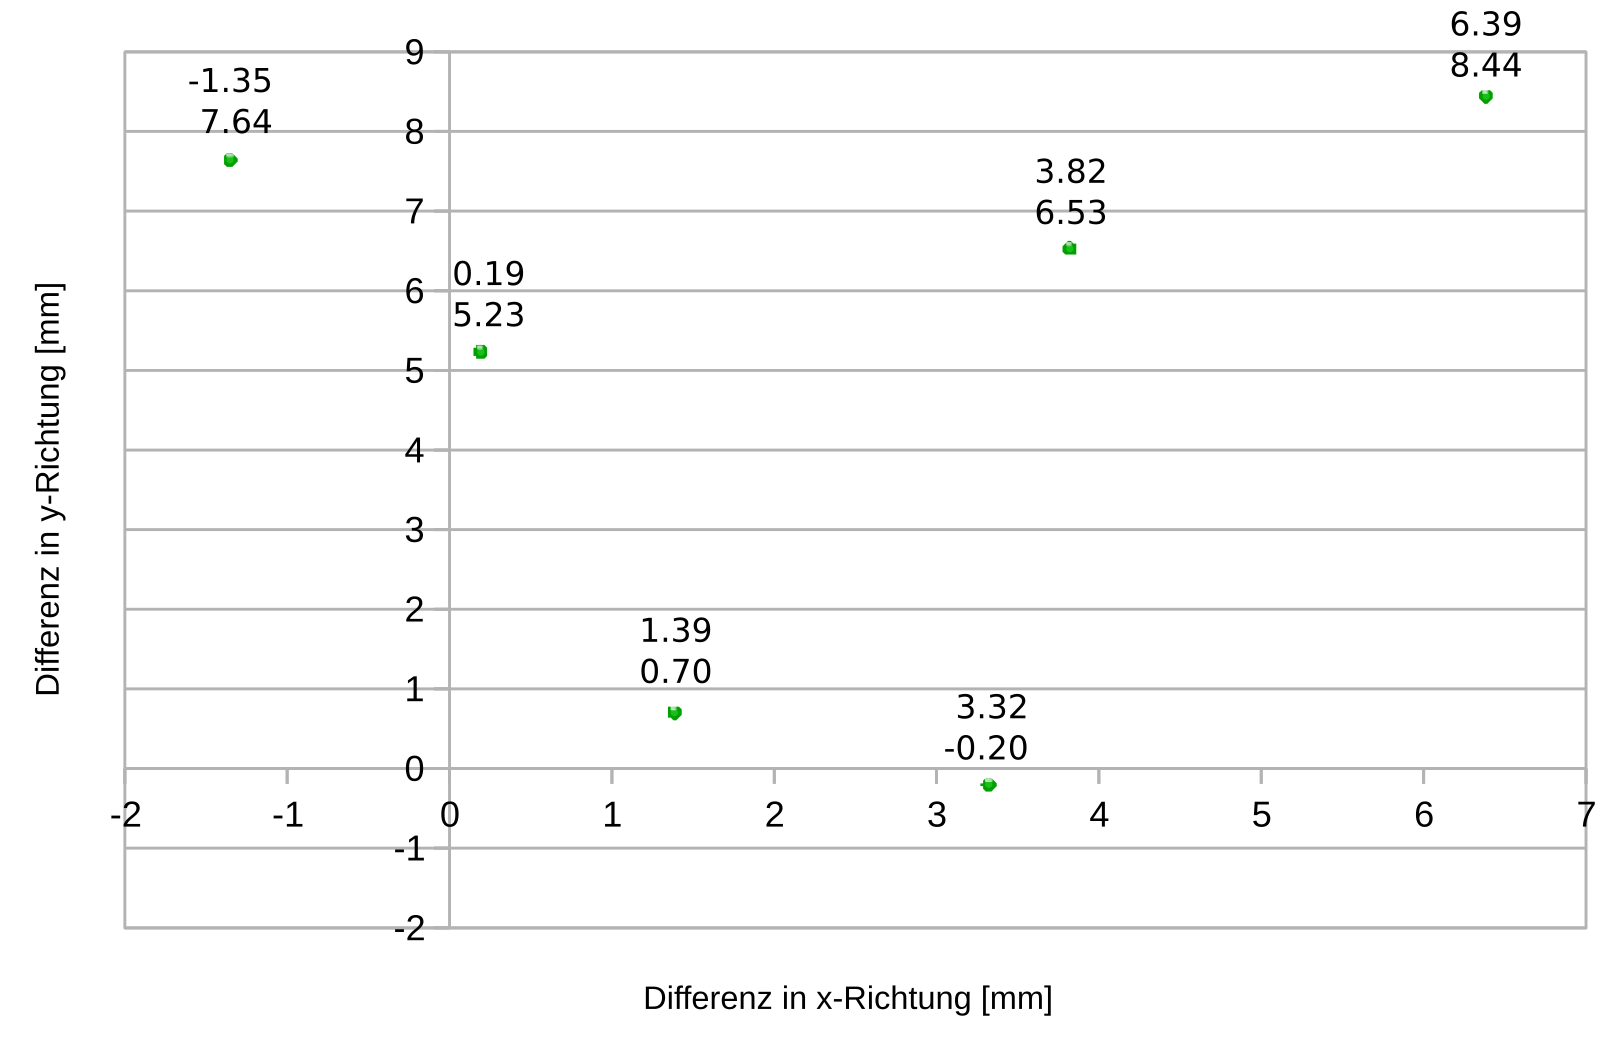
\includegraphics[width=0.88\textwidth]{images/ergebnisse/Differenzen_beim_Teachen_mit_Gesten}
	\caption[Positionsdifferenzen beim Teachen mit der Roboter-Gesten-Anwendung]{Positionsdifferenzen beim Teachen mit der Roboter-Gesten-Anwendung\\Quelle: Eigene Ausarbeitung}
	\label{fig:measurement_teaching_positions}
\end{figure}
\FloatBarrier

\textcolor{red}{TODO}

\begin{figure}[htb]
	\centering
	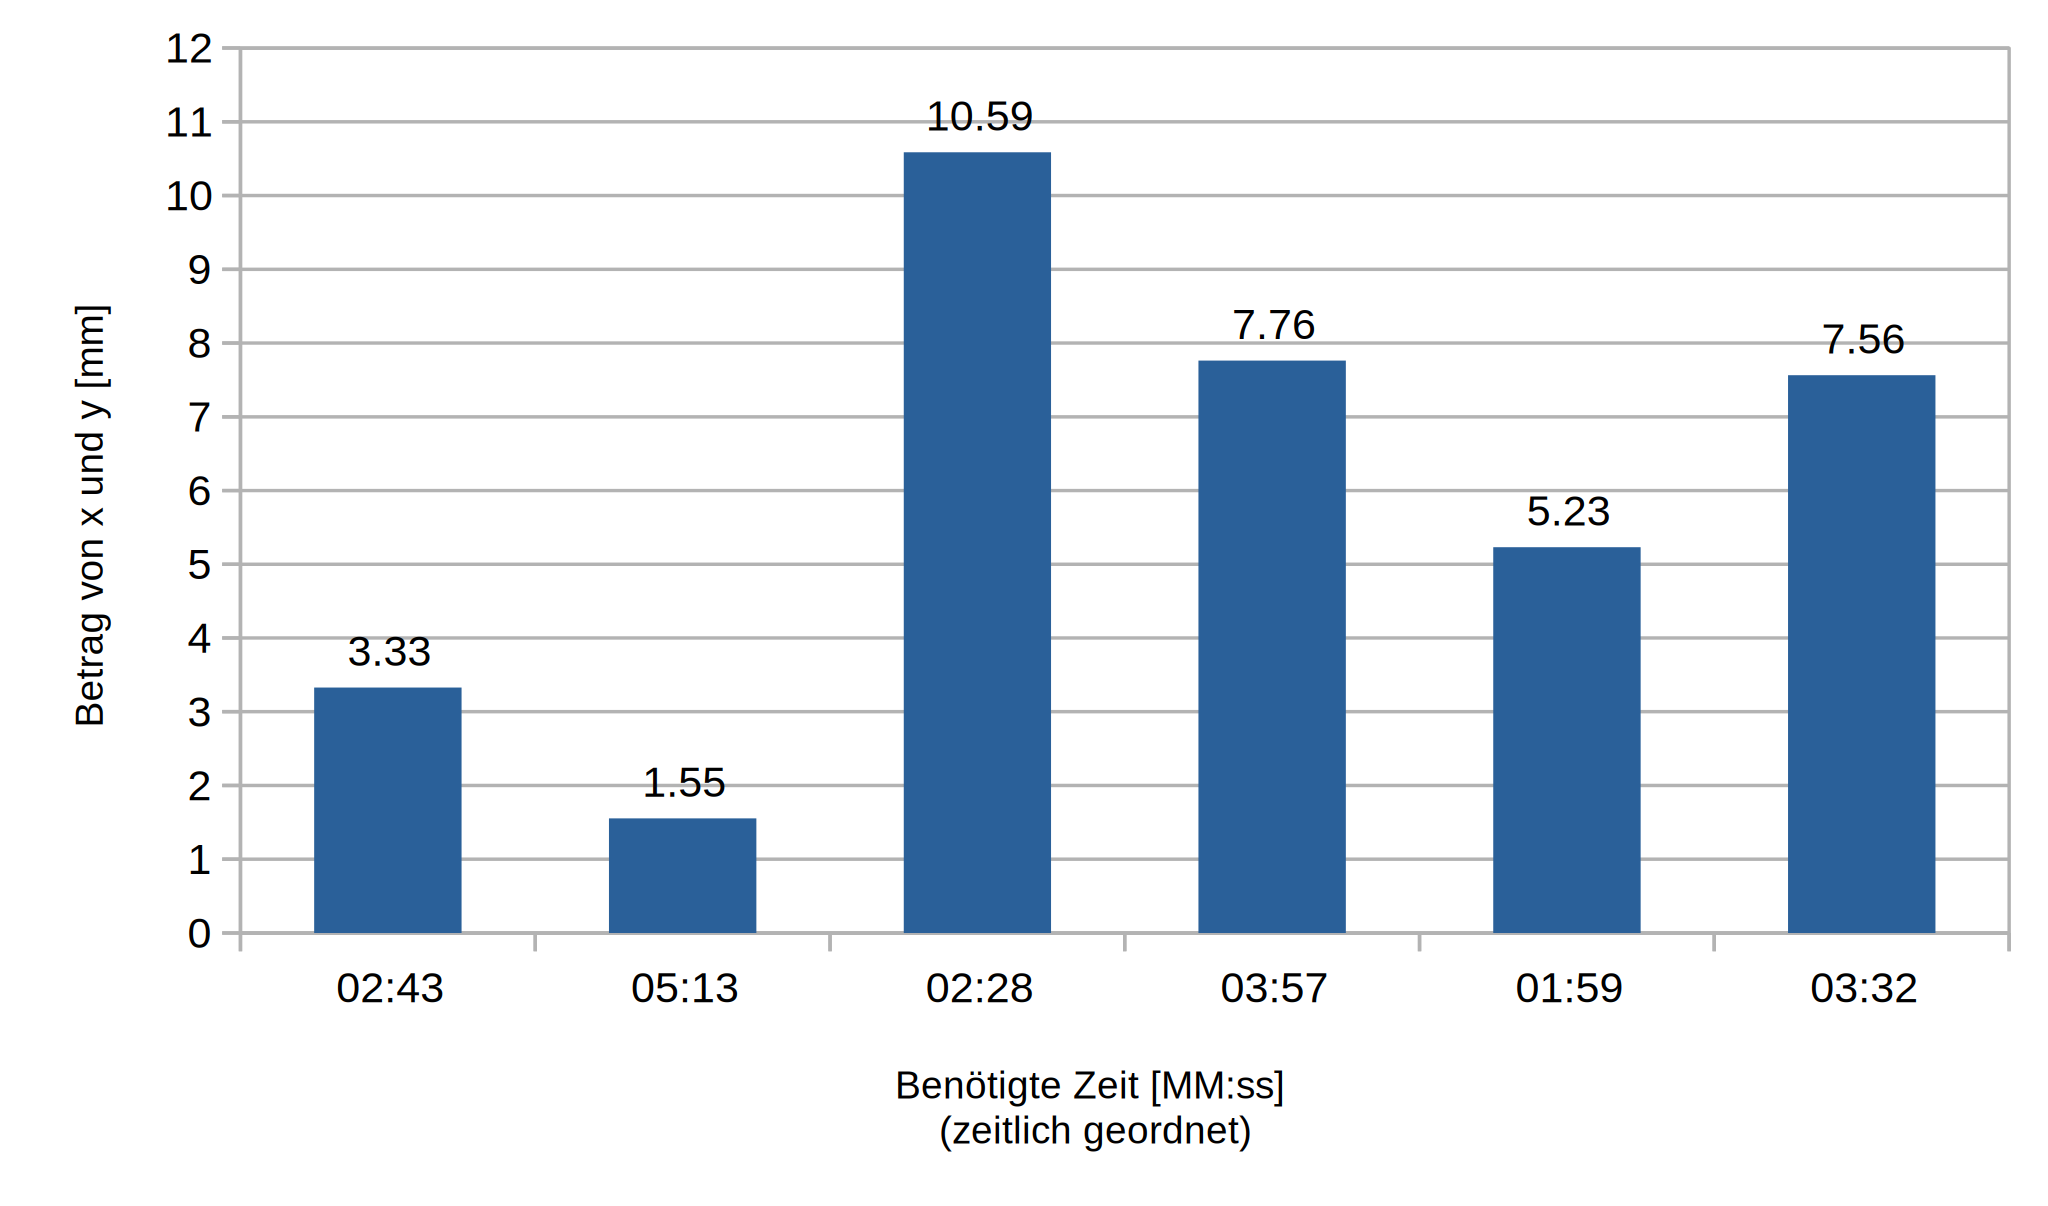
\includegraphics[width=0.88\textwidth]{images/ergebnisse/Betrag_der_Fehlerquadrate}
	\caption[Betrag der Fehlerquadrate beim Teachen mit der Roboter-Gesten-Anwendung]{Betrag der Fehlerquadrate beim Teachen mit der Roboter-Gesten-Anwendung\\Quelle: Eigene Ausarbeitung}
	\label{fig:measurement_teaching_positions}
\end{figure}
\FloatBarrier

\textcolor{red}{TODO}

\section{Genauigkeit der Gestenerkennung}
% Wie viele Versuche benötigt ein Proband bis seine Gesten erkannt werden?

% \section{Ergonomie \& User Experience}
% Verbessert dieser Ansatz die Ergonomie des Teachen in eine positive Richtung?
% Ist es angenehmer diese NUI-Methode zu verwenden als ein herkömmliches Teach Pendant?
% Kann ich über eine längere Zeitspanne, wie z.B. 30 Minuten, einen Roboter teachen?
% Wie schnell bin ich erschöpft im Gegensatz zu einem herkömmlichen Teach Pendant?
% Wie schnell erlernt man die Gesten?
% Wie einprägsam sind die Gesten?
% Sind die Gesten gut geeignet um einen Roboter zu steuern oder sind diese zu schwammig oder zu ähnlich und werden daher auch oft verwechselt?
%   * Können diese im besten Fall nur schwer unbeabsichtigt durchgeführt werden und fälschlicherweise nicht z.B. als kulturelle Geste erkannt werden?
%   * Gibt es wenige Überschneidungen mit bereits definierten Gesten, sodass diese nicht unbeabsichtigt durchgeführt werden können?
%   * Sind diese leicht anzuwenden, sodass das System die Geste im besten Fall beim ersten Mal erkennt?

% Erkennungsrate der Gestenerkennung

\textcolor{red}{TODO:\\
Wie gut ist das System einsetzbar? UX\\
Bewertung der Ergonomie über längere Zeitdauer (sehr subjektiv, jedoch aber versuchen die Ergebnisse auf die Allgemeinheit zu bezienen)\\
Während dem Teachen bewegt man sich oft um zu sehen ob der Endeffektor an der richtigen Stelle ist. Mit einer fest angebrachten Azure Kinect ist es daher schwer den eigenen Blickwinkel zu ändern\\
reflexartige und unbeabsichtigte Bewegungen\\
Beim Teachen steht man normalerweise um den Roboter ordnungsgemäß und vollständig sehen zu können
% siehe 3.4.3 Auswahl anhand der Ergonomie
}

% muss nicht auf die Körpergröße eingestellt werden, da der Field of View sehr groß ist

% Kann ich über eine längere Zeitspanne, wie z.B. 30 Minuten, einen Roboter teachen? Wie schnell bin ich erschöpft im Gegensatz zu einem herkömmlichen Teachpendant? Wie schnell lernt man die Gesten? Sind die Gesten gut geeignet um einen Roboter zu steuern oder sind diese zu schwammig oder zu ähnlich und werden daher auch oft verwechselt?
